\section{Water Treatment}
The following treatment train was chosen for regenerating water from human waste streams.
\begin{figure}[h!]
    \centering
    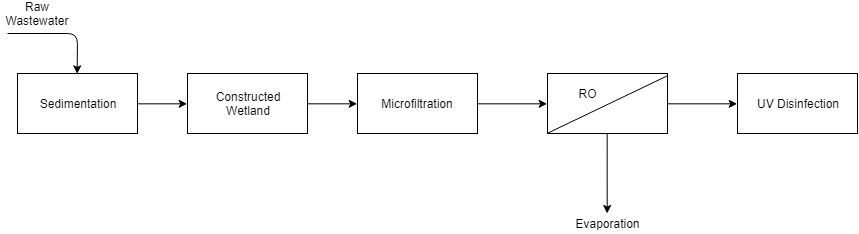
\includegraphics[width=0.75\textwidth]{treatment_train}
    \caption{Wastewater treatment train}
    \label{fig:treatment_train}
\end{figure}
\subsection{Sedimentation}
To model the sedimentation of particles in the pre-treatment basin, a simple set of equations is used \cite{principles}. To model the settling velocity of particles:
\begin{align}
    v_s &= \frac{g(\rho_p - \rho_w)d_p^2}{18\mu} & \text{Re $< 2$} \;\; \text{(laminar flow)} \\
    v_s &= \left[ \frac{g(\rho_p - \rho_w)d_p^{1.6}}{13.9\rho_w^{0.4} \mu^{0.6}} \right]^{1/1.4} & \text{$2 \leq$ Re $\leq 500$} \;\; \text{(transition flow)}
\end{align}
where
\begin{equation}
    \text{Re} = \frac{\rho_w v_s d_p}{\mu} = \frac{v_s d_p}{\nu}
\end{equation}
and
\begin{conditions*}
    v_s & Settling velocity of the particle (m/s) \\
    g & Acceleration due to gravity, 9.81 m/s$^2$ \\
    \rho_p & Density of the particle (kg/m$^3$) \\
    \rho_w & Density of water (kg/m$^3$) \\
    C_d & Drag coefficient, unitless \\
    d_p & Diameter of particle (m) \\
    \text{Re} & Reynolds number, dimensionless \\
    \mu & Dynamic viscosity (N$\cdot$s/m$^2$) \\
    \nu & Kinematic viscosity (m$^2$/s)
\end{conditions*}
Based off the particle velocity and properties of the water, the sedimentation basin dimensions can be calculated so that all particles with a diameter greater than $D$ (i.e. $d_p \geq D$) will be fully removed. To do so, the following equation is used:
\begin{equation}
    v_D = v_c = \frac{h_0}{\tau} = \frac{h_0Q}{h_0A} = \frac{Q}{A} \implies A = \frac{Q}{v_D}
\end{equation}
where 
\begin{conditions*}
    v_D & Settling velocity of particle with diameter $D$ (m/s) \\
    v_c & Critical velocity such that particle at surface of inlet is removed just before outlet (m/s) \\
    h_0 & Height of the sedimentation basin (m) \\
    \tau & Hydraulic retention time in basin (s) \\
    Q & Sedimentation basin loading rate (m$^3$/s) \\
    A & Sedimentation basin area (m$^2$)
\end{conditions*}
Once the area is calculated, the length, width, and depth can be determined using a preferential L:W ratio of 5:1 and a preferential depth of 4 m \cite{principles}.\\\\
The fraction of particles removed for a specific diameter less than $D$, the following equation can be used:
\begin{equation}
    \text{Fraction of particles removed} = \frac{v_s}{v_D}\,(v_s<v_D)
\end{equation}
\subsection{Wetlands Treatment}
%\subsubsection{Modeling Parameters}
%If not available from the literature, the following equation was used to model the wetland's hydraulic conductivity \cite{Ks_estimate}:
%\begin{equation}
%    K_s=0.24622\,[d_{10}^2\varepsilon^3/(1+\varepsilon)]^{0.7825}
%\end{equation}
%where
%\begin{conditions*}
%K_s & Saturated hydraulic conductivity (m/s) \\
%d_{10} & 10th-percentile particle size (mm) \\
%\varepsilon & Void fraction/porosity of bed
%\end{conditions*}
\subsubsection{Green-Ampt Modeling}
The Green-Ampt equation \cite{green_ampt} is used to model infiltration into a vertical constructed wetland. For a one-layer wetland, the following equation is used to calculate the time to saturate the wetland with or without ponding at the surface\footnote{Note: For consistency, $\Psi < 0$ and $h_0 \geq 0$. Thus, $\Delta h$ will always be $\geq 0$.}.
\begin{gather}
\label{eq:t_1}
    t_1=\frac{\theta_s - \theta_i}{K_s}\left[z_1 - \Delta h \ln{\left(1+\frac{z_1}{\Delta h}\right)}\right] \\
\label{eq:delta_h}
      \Delta h = h_0 - \Psi_f \\ 
\label{eq:theta_i}
  \theta_i \approx \theta_{fc} = \phi\left(\frac{|\Psi_{ae}|}{340}\right)^\frac{1}{b} \\
\label{eq:Psi_f}
    |\Psi_f| \approx \frac{|\Psi_{ae}|}{2}
\end{gather}
where
\begin{conditions*}
    t_1 & Time to saturate one-layer wetland (hr) \\
   \theta_s & Saturated water content (= to porosity $\phi$) \\
    \theta_i & Initial water content\footnote{Equation for soil field capacity is used to represent a "dry" soil after first wetting. $\theta_i$ can be set to 0 for first wetting.} \\
    \theta_{fc} & Soil field capacity, i.e. the water content held against gravity\footnote{Derived from \cite{garcia_7}.} \\
    K_s & Saturated hydraulic conductivity (m hr$^{-1}$) \\
   z_1 & Depth of the wetland basin (m) \\
    \Delta h & Pressure head difference (m) \\
    \Psi_f & Suction head of the wetting front (m)\footnote{This approximation is established in \cite{green_ampt}.} \\
    \phi & Porosity of the material
\end{conditions*}
%For a two-layer system, the total time $t$ is calculated using the following equation \cite{green_ampt}:
%\begin{equation}
%\label{eq:t_2}
%    t = t_1 + \frac{\theta_{s,2}-\theta_{i,2}}{K_{s,2}}
%    \left[ z-z_1+\left(\frac{z_1K_{s,2}}{K_{s,1}}-z_1-\Delta h\right)\ln{\left(\frac{z+\Delta h}{z_1+\Delta h}\right)}\right]
%\end{equation}
%where 
%\begin{equation*}
%    \Delta_h = h_0 - \Psi_{f,2}
%\end{equation*}
%and values for $t_1$, $\theta_i$, and $\Psi_f$ are calculated using \eqref{eq:t_1}-\eqref{eq:Psi_f}.
\subsection{Treatment Kinetics}
%Using $t$ as an estimate for hydraulic residence time (HRT), the system can be modeled as an ideal plug-flow reactor for modeling degradation of COD, BOD, TSS, NH$_4$, and TP using rate constants derived from \cite{pilot} and the following equation:
Kinetics are modeled using the $P-k-C*$ model of \cite{kadlec} with areal rate constants derived from \cite{kA}:
\begin{equation}
    \frac{C-C^*}{C_i-C^*}=\left(1+\frac{k_Ay}{Pq}\right)^{-P}
\end{equation}
where
\begin{conditions*}
    C & Concentration at $y$ (mg/L) \\
    C_i & Concentration at inlet (mg/L) \\
    C^* & Background concentration (mg/L) \\
    k_A & Areal rate constant (m/day) \\
    y & Depth in wetland (m) \\
    P & apparent number of TIS\footnote{TIS = Tanks in series. For our model, $P=1$, i.e. a plug-flow system.}
\end{conditions*}
Values for $k_A$ are summarized below (Table \ref{tab:kA}) for a wetland packed with 0-4 mm gravel ($d_{10}=0.55$mm, $d_{60}=3.1$mm) and planted with common reed plants (\textit{Phragmites australis}).
\begin{table}[ht]
    \centering
    \begin{tabular}{c|c}
    \textbf{Pollutant} & \textbf{$k_A$ (m/day)} \\
    \hline
    BOD$_5$ & 0.43 \\
    TSS & 0.28 \\
    NH$_4^+$ & 0.56
    \end{tabular}
    \caption{$k_A$ rate constants from \cite{kA}}
    \label{tab:kA}
\end{table}
\subsection{Filtration}
\subsubsection{TSS Removal}
While the rate constants above can only be verified through experimentation, the rate of removal of TSS can be estimated using an independent set of equations if we consider the wetland equivalent to a rapid granular filter. This will serve to verify, perhaps, the $k_A$ value from Table \ref{tab:kA}.

Yao et al. developed a model of water filtration based off filter media grains acting as collectors for particles which enter their region of influence. The mass removal is calculated as the rate at which particles enter their proximity multiplied by a transport efficiency ($\eta$) and attachment efficiency factor ($\alpha$). The mass balance was developed by Crittenden et al. to be modeled as a first-order reaction \cite{principles}.
\begin{equation}
    \frac{dC}{dz} = \left(\frac{-3(1-\varepsilon)\eta\alpha}{2d_C}\right)C \implies
    \text{i.e.}\;\; C =C_0 \exp{\left[\frac{-3(1-\varepsilon)\eta\alpha L}{2d_C}\right]}
\end{equation}
where
\begin{conditions*}
    C,C_0 & Concentration of suspended solids (mg/L) \\
    \varepsilon & Wetland bed porosity \\
    \eta & Transport efficiency factor, unitless \\
    \alpha & Attachment efficiency factor, unitless \\
    L & Wetland bed depth (m) \\
    d_C & Diameter of wetland bed media (m)
\end{conditions*}
The process for calculating the transport efficiency are described below. For this experiment, the attachment efficiency is assumed to be 1.0 \cite{principles}.

Transport efficiency is divided into three primary influences: diffusion ($\eta_D$), accounting for the Brownian motion of particles which causes them to deviate from their flow path; sedimentation ($\eta_G$), which causes larger particles to more often deviate from their flow path due to gravitational forces; and interception ($\eta_I$), which causes particles passing within half a diameter of filter particles to be intercepted.
\begin{gather}
    \eta = \eta_D + \eta_G + \eta_I \\
    \eta_D = 2.4\,A_S^{1/3}N_R{-0.081}N_V^{0.052}\text{Pe}^{-0.715} \\
    \eta_G = 0.22\,N_R^{-0.24}N_V{0.053}N_G^{1.11} \\
    \eta_I = 0.55\,A_S N_A^{1/8}N_R^{1.675}
\end{gather}
where
\begin{conditions*}
    \eta_D & Transport efficiency due to diffusion, dimensionless \\
    \eta_G & Transport efficiency due to gravity, dimensionless \\
    \eta_I & Transport efficiency due to interception, dimensionless \\
    A_S & Porosity parameter that accounts for the effect of adjacent media grains, dimensionless \\
    N_R & Relative size number, dimensionless \\
    N_V & van der Waals number, dimensionless \\
    \text{Pe} & Peclet number, dimensionless \\
    N_G & Gravity number, dimensionless \\
    N_A & Attraction number accounting for attraction between collector and particle as the particle gets closer, dimensionless
\end{conditions*}
The dimensionless numbers above can be calculated as follows:
\begin{gather}
    A_S = \frac{2(1-\gamma^5)}{2-3\gamma+3\gamma^5-2\gamma^6} \\
    N_R = \frac{d_p}{d_C} \\
    N_V = \frac{\text{Ha}}{k_B T} \\
    \text{Pe} = \frac{3\pi\mu d_p d_C v_F}{k_B T} \\
    N_G = \frac{v_S}{v_F} = \frac{g(\rho_P-\rho_W)d_p^2}{18\mu v_F} \\
    N_A = \frac{N_V}{N_R \text{Pe}} = \frac{\text{Ha}}{3\pi\mu d_p^2 v_F}
\end{gather}
where
\begin{conditions*}
    \gamma & $(1-\varepsilon)^{1/3}$, dimensionless \\
    \varepsilon & Wetland bed porosity, dimensionless \\
    d_p, d_C & Particle and collector diameters (m) \\
    \text{Ha} & Hamaker constant, J \\
    k_B & Boltzmann constant, $1.381\times 10^{-23}$ J/K \\
    T & Absolute temperature (K) \\
    \mu & Water dynamic viscosity (Pa-s) \\
    v_F & Superficial velocity of particles (m/s)\footnote{This is set equal to the hydraulic loading rate $q$ in the simulation.} \\
    v_S & Stokes settling velocity (m/s) \\
    g & Gravitational constant, 9.81 m/s$^2$ \\
    \rho_p,\rho_W & Density of particles and water (kg/m$^3$)
\end{conditions*}
\subsubsection{Head Loss}
Clean bed head loss due to inertial and viscous forces can be estimated using the Ergun equation \cite{principles}:
\begin{equation}
\label{eq:ergun}
    h_L=\kappa_V\frac{(1-\varepsilon)^2}{\varepsilon^3}\frac{\mu Lv_F}{\rho_W gd^2} + \kappa_I \frac{1-\varepsilon}{\varepsilon^3}\frac{Lv_F^2}{gd}
\end{equation}
where
\begin{conditions*}
    h_L & Head loss in clean bed (m) \\
    \kappa_V,\kappa_I & Ergun coefficients for viscous and inertial losses, unitless \\
    \varepsilon & Filter bed porosity \\
    L & Filter bed length (m) \\
    v_F & Superficial velocity of particles (m/s)\footnote{This is set equal to the hydraulic loading rate $q$ in the simulation.} \\
    \mu & Water dynamic visocity (Pa-s) \\
    \rho_W & Water density (kg/m$^3$) \\
    g & Gravitational coefficient (9.81 m/s$^2$) \\
    d & Diameter of bed media (m)
\end{conditions*}
\subsection{Assumptions}
The main assumptions for the treatment wetlands are:
\begin{itemize}
    \item The assumptions of the Green-Ampt equation including a sharp wetting front and complete saturation of the wetted area.
    \item The wetland behaves like an ideal plug-flow reactor.
    \item The wetlands are packed with 0.8m of 0-4 mm gravel and densely packed with common reed.
    \item Particle size distribution of raw wastewater follows that of \cite{particle_size_dist} (Table \ref{tab:particle_size_dist}).
\end{itemize}
\begin{table}[ht]
    \centering
    \begin{tabular}{l|l}
    Particle fraction ($\mu$m) & Prevalence in wastewater (\%)  \\
    \hline
    $d_p \leq$ 12 & 26 \\
    $12 < d_p \leq 63$ & 27 \\
    $63 < d_p \leq 1000$ & 33 \\
    $d_p > 1000$ & 14
    \end{tabular}
    \caption{Particle size distribution in raw wastewater}
    \label{tab:particle_size_dist}
\end{table}
In reality, none of the assumptions above would likely hold true and thus, this is a heavily idealized system used to model an approximation of treatment quality and hydraulic characteristics.
